
\chapter{Practical Experiments}
\label{ch:inpractice}

This chapter shows two experiments and their results of an advanced use of the Zone. The first realizes an asynchronous sequence diagram of a parallel program with dependencies. The second describe how to transparently instrument the third-party framework \vertx\ to realize a ``Zone-aware \vertx''.

\section{Asynchronous Sequence Diagram}


\paragraph{Specifying} what is interesting in an asynchronous sequence diagram is the most complex part if this experiment. In fact, producing the information of a conventional sequence diagram is not interesting. There are already many tools to do that. The useful data is an asynchronous dependency diagram: what are the dependencies between asynchronous tasks. The produced diagram is defined by:

\begin{itemize}
\item Each task execution is divided into sub parts, represented by the nodes of a graph.
\item Tasks are divided into the biggest possible parts such that a sub-part execution first uniquely shows \emph{incoming} dependencies (rely on other tasks result or completion). Then it uniquely shows \emph{outgoing} dependencies (another task shows incoming dependency from this task).
\item Dependencies are represented as directed edges between the corresponding nodes of their tasks.
\end{itemize}

The produced graph is a directed acyclic graph where each node represents an autonomous part of the programs and the edges show the precedences between those parts.

\paragraph{The realization} is then pretty easy using the Zone. As evoked in chapter \ref{ch:apps}, use the one Zone per task pattern, creating \lstinline{TaskZone}s. Each \lstinline{TaskZone} stores a unique task ID and defines the crossing hook: 

\begin{lstlisting}
// The cross operation executes inside -destination- Zone

// The cross operation is defined inside -source- Zone

public Token crossOut(Token token) {
  TaskZone sourceZone = this;
  int sourceID = sourceZone.taskId;

  int destID = Zone.lookup(TASK_ID_KEY);

  storeDependency(souceID, destID);
}
\end{lstlisting}

The difficult part is then to compile collected information and build a graphical representation. For the code of a fork-join algorithm (figure \ref{fig:fj-alg}) I used a sample code from the d3.js library to produce the view shown in figure \ref{fig:fjt-bundle}. Each node is named 'X\#Y'. 'X' is the task id and 'Y' the subtask id. The initial task is '0', split in two subtasks '0\#1' entry point of algorithm and '0\#2', end of the algorithm with output value.

\begin{figure}[h]
  \textbf{Solving problem $P$}
  \begin{enumerate}
  \item If $P$ is small then solve $P$.
  \item Else split $P$ in a list $P$s of smaller problems $p$.
  \item For each $p$ in $P$s, start an asynchronous task to solve $p$.
  \item Join each asynchronous task started in (3) and collect all sub-results.
  \item Compose the sub-results and return the final solution.
  \end{enumerate}
\caption{Generic fork-join algorithm}
\label{fig:fj-alg}
\end{figure}

\begin{figure}
  \centering
  \makebox[\textwidth][c]{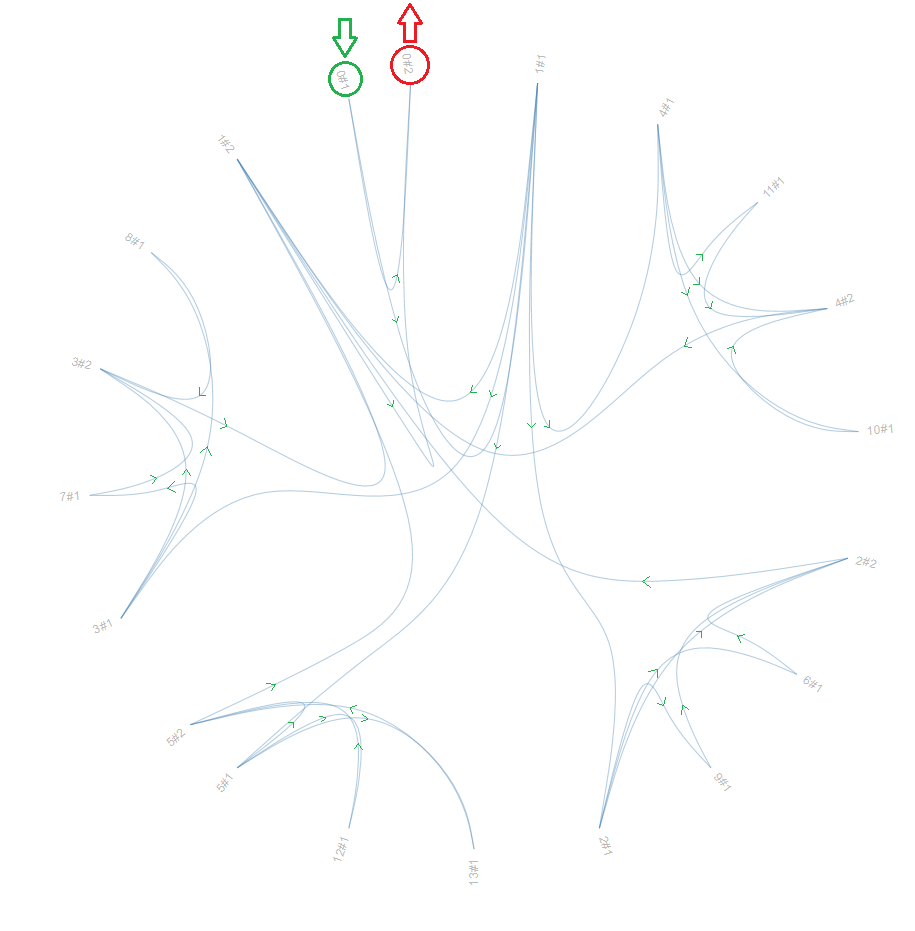
\includegraphics[width=1.4\textwidth]{bundle-fjt}}
  \caption{Fork-join algorithm dependency graph}
  \label{fig:fjt-bundle}
\end{figure}


\section{Transparent Instrumentation}

In this experiment, I used the AOP framework AspectJ to automatically instrument the \vertx\ library. If analyzing the \vertx\ code to define where and how to apply the Zone was tedious, the concrete realization was much simpler.

\paragraph{Results} of this work are:
\begin{itemize}
\item Integration code is quite small (only six classes of 60 lines in average).
\item Aspect weaving only relies on public \vertx\ API and assumes no internal behavior.
\item The instrumentation is done by a stand-alone program that produce an artifact interchangeable with the original \vertx.
\end{itemize}

``Interchangeable'' here means one can transparently be replaced by the other. If used on an existing project, the only thing to modify is the import resolution in the project configuration. Since the instrumented \vertx\ library completely reproduces the original package structure, the imports in the different classes do not need modification.

With this instrumented library, I was even able to reuse the classes developed for the asynchronous dependency diagram to visualize the dependencies of a \vertx\ program.


